\section{Modeling \pp collisions}
In collisions at very low energies, protons can be approximated as electrically charged objects. At higher energies, such as those at the LHC, the structure within protons begins to have an important role for the scattering process. \W and \Z bosons are produced from the interaction of quarks and gluons (both also referred to as partons) within the proton\cite{PhysRevLett.23.930,PhysRevLett.23.935}. The contributions of the partons to the proton's structure are described by parton distribution functions (PDFs). The PDFs cannot be calculated directly, and are instead determined from experimental data.  (add citations) Valence quarks, sea quarks, and gluons within the proton are described by the PDFs. 
% Therefore, the internal structure of the protons is represented by the structure functions i.e. in Equation~\ref{eq:structure_func}, where the $x$ is the fraction of the proton's total momentum carried by a given parton, and $f_i(x)$ is the distribution of the parton. 
% \begin{equation}
% F(x) = \sum_i{x_if_i(x_i)}
    % \label{eq:structure_func}
% \end{equation}

Calculations for cross section predictions must be done perturabitively in QCD. The highest order calculation currently available for the \W and \Z production is NNLO
\cite{Anastasiou:2003ds}. However, soft and collinear gluons emissions produce logarithmic terms which cause singularities. The factorization theorem can be used in QCD processes, separating the perturbative and non-perturbative sections of the calculation at a factorization scale, $\mu_F$~\cite{Collins:1989gx}. This allows the singularities due to the soft gluon emissions to be factored out and contained within the PDFs.  Equation~\ref{eq:factorization_xsec} shows the factorized cross section calculation. $f_{a}$ and $f_{b}$ are the parton distribution functions for the quarks and gluons in the two protons, $x_a$ and $x_b$ are the fractions of total momentum carried by each parton, and $\hat{\sigma}$ is the cross section for the hard process. 

\begin{equation}
\begin{aligned}
\sigma_{p_a p_b \rightarrow n} &= \sum_{a,b}{\int{dx_a dx_b f_{a}(x_a, \mu^2_F)f_{b}(x_b, \mu^2_F)}} \\ &\times[\hat{\sigma}_{LO}(x_a x_b s, \mu^2_R, \mu^2_F)+\alpha_S \hat{\sigma}_{NLO}(x_a x_b s, \mu^2_R, \mu^2_F) + \cdot]
    \label{eq:factorization_xsec}
\end{aligned}
\end{equation}
Factorization scale dependence of the PDFs is determined by the DGLAP equation. Parametrizations of PDFs are determined, and solutions to the DGLAP equation provide the evolution of the PDFs over different scales of $\mu_F$ \cite{Gribov:1972ri,Dokshitzer:1977sg}

\begin{figure}
\centering
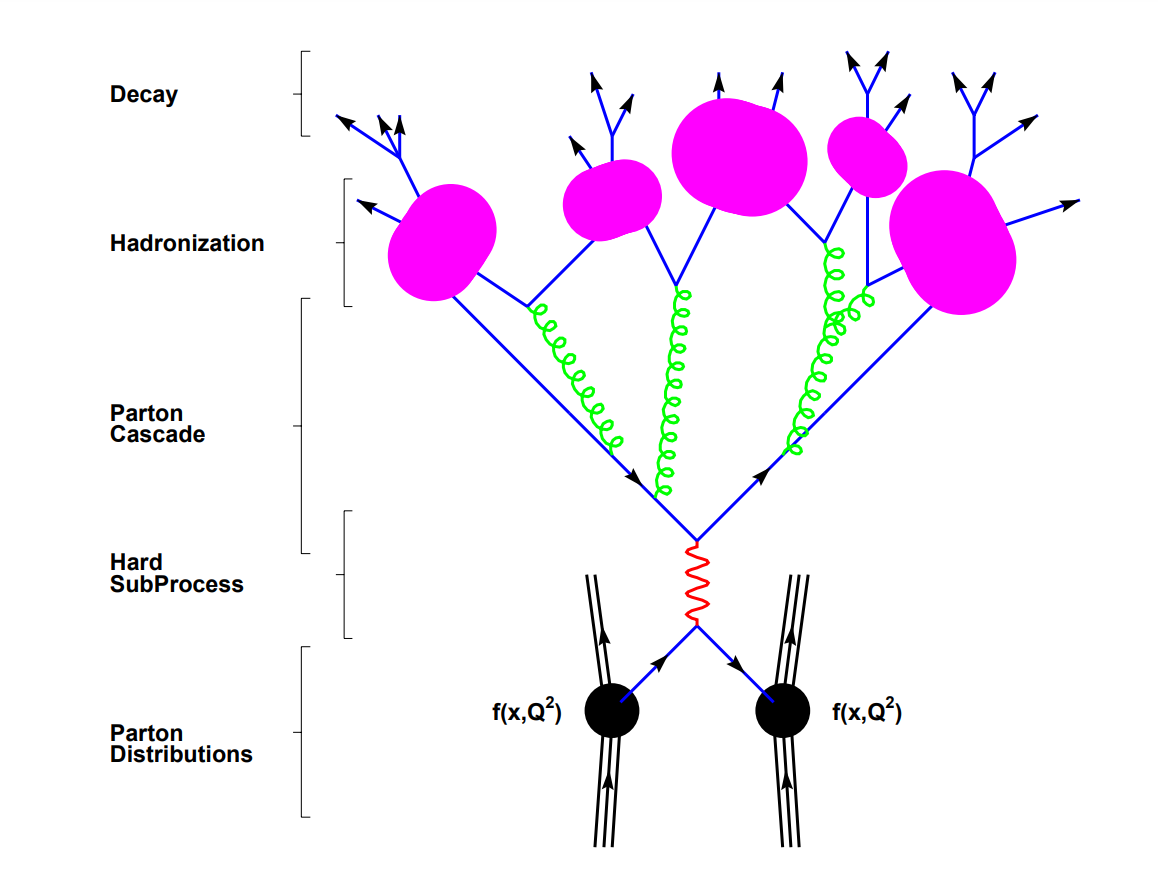
\includegraphics[width=0.6\linewidth]{plots/SM/evtgenerator.PNG}
%   \caption{1a}
%   \label{fig:Eff:el:5TeV:GSFSel:pos
\caption{Illustration of a hard-scatter process. \protect\cite{Dobbs:2001ck}}
\label{fig:sm:evtgen}
\end{figure}

Matrix element calculation breaks down for soft and collinear final states. Instead, parton shower models are used to produce the final-states at non-perturbative scales. Showering is modeled as series of radiative steps, with partons branching into consecutively lower energy state: $q\rightarrow gq$, $g\rightarrow gg$, and $g\rightarrow q\bar{q}$ for QCD. Additionally QED interactions ($q\rightarrow q\gamma$ and $l\rightarrow l\gamma$) are included in the shower modeling. Parton showering continues to the scale $\Lambda_{QCD}\approx 200~\mathrm{MeV}$, bare partons are hadronized into color-neutral hadrons. Then the unstable hadrons are decayed according to branching ratios. Factorization and a hard scatter process, along with subsequent parton showering and hadronization is illustrated in Figure~\ref{fig:sm:evtgen}.



\subsection{\W and \Z production at the LHC [need some work]}
In the \pp collisions, the bosons are produced through the interaction of quarks and gluons within the protons \cite{}. The primary production modes for the \W and \Z bosons is through the Drell-Yann process, predonminantly $u\bar{u}, d\bar{d}\rightarrow Z$,  $u\bar{d}\rightarrow W^+$,  and $d\bar{u}\rightarrow W^-$. 

Figure~\ref{fig:sm:summary:xVsQ2}.

%%%% figure
\begin{figure}
\centering
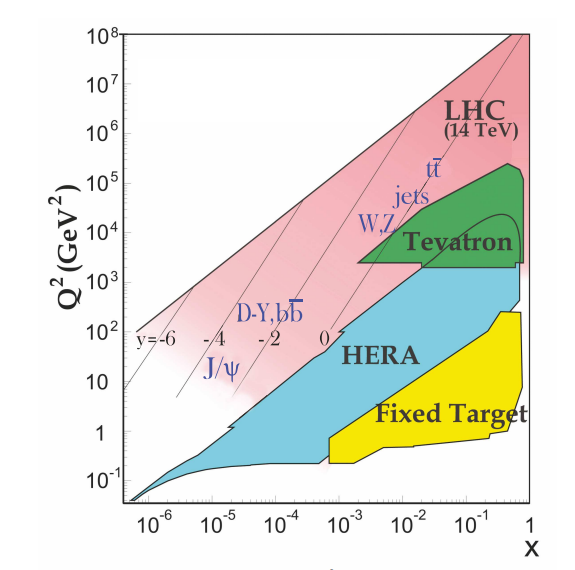
\includegraphics[width=0.6\linewidth]{plots/SM/structure_probes.PNG}
%   \caption{1a}
%   \label{fig:Eff:el:5TeV:GSFSel:pos
\caption{Phase space of Bjorken-x and $Q^2$ available at the LHC and other experiments. \pp collisions at the LHC can probe very high $Q^2$. \protect\cite{PhysRevD.98.030001}}
\label{fig:sm:summary:xVsQ2}
\end{figure}



\subsection{Simulating \pp collisions[need some work]}
Practical descriptions of theoretical predictions are provided by Monte Carlo event generators. These generators rely on the approximations and factorization schemes that were described earlier in this section. Many collaborations dedicated to event generation tools exist, and are important in the era of LHC physics. The event generators come in generally two types: matrix element generators and parton shower generators. The matrix-element generators are distinguished by the order in $\alpha_s$ to which they provide calculations. 
\begin{itemize}
    \item \textbf{Pythia}: Pythia is a general-purpose event generator and can do both matrix-element calculation as well as initial and final state radiation and multiparton interactions. Pythia is often interfaced to other matrix-element calculators, where it provides the parton showering and hadronization steps, as done for the samples used in this analysis. \cite{Sjostrand:2014zea}
    \item \textbf{aMC@NLO} MadGraph5\_aMC@NLO is a generator which provides matrix element calculations with up to two additional partons in the final state. This uses the NNPDF3.1 NLO PDF set.
    \item \textbf{ResBos} 
    \item \textbf{Powheg}
\end{itemize}


Predictions from event generators have uncertainties from several sources. Low-energy QCD processes which are dominiated by non-perturabtive effects are not well modeled and have large uncertainties. Parton showering is limited by its reliance on approximations. Proton PDFs have uncertainties. Additional uncertainty comes from higher-order terms in both QCD and QED, which are currently used at NNLO and LO. 

PDF  uncertainties - general comment
include multiple error sets reflecting the best fit with 1 sigma variations on the all of the params in the fit
reflect uncertainties in data also
inherent systematics dependent on way global fit is set up


better predicionts of ewk mixing angle, w mass etc
